%15 min preso!
\documentclass[xcolor=table,aspectratio=169]{beamer}
\usepackage{beamerthemesplit}
\usepackage{wrapfig}
\usetheme{SPbGU}
\usepackage{pdfpages}
\usepackage{amsmath}
\usepackage{cmap}
\usepackage[T2A]{fontenc}
\usepackage[utf8]{inputenc}
\usepackage[english]{babel}
\usepackage{indentfirst}
\usepackage{amsmath}
\usepackage{tikz}
\usepackage{multirow}
\usepackage[noend]{algpseudocode}
\usepackage{algorithm}
\usepackage{algorithmicx}
\usepackage{fancyvrb}
\usepackage{hyperref} 
\usetikzlibrary{calc}
\usetikzlibrary{shapes}
\usetikzlibrary{arrows,automata}
\usetikzlibrary{positioning}
\usetikzlibrary{fit}
\usetikzlibrary{shapes.callouts}
\usetikzlibrary{shapes.misc}
\usepackage{xparse}

\usepackage{etoolbox,refcount}
\usepackage{multicol}

\usepackage{fontawesome5}
\usepackage{fontawesome}

\usepackage{tabularx}
\newcolumntype{Y}{>{\raggedleft\arraybackslash}X}

\renewcommand{\thealgorithm}{}

\newtheorem{mytheorem}{Theorem}
\renewcommand{\thealgorithm}{}

\newcommand{\tikzmark}[1]{\tikz[overlay,remember picture] \node (#1) {};}
\def\Put(#1,#2)#3{\leavevmode\makebox(0,0){\put(#1,#2){#3}}}

\newcommand{\ltz}{$< 1$}

\tikzset{
    state/.style={
           rectangle,
           rounded corners,
           draw=black, very thick,
           minimum height=2em,
           inner sep=2pt,
           text centered,
           },
}

\tikzset{
    invisible/.style={opacity=0,text opacity=0},
    visible on/.style={alt=#1{}{invisible}},
    alt/.code args={<#1>#2#3}{%
      \alt<#1>{\pgfkeysalso{#2}}{\pgfkeysalso{#3}} % \pgfkeysalso doesn't change the path
    },
}

\tikzset{cross/.style={cross out, draw=black, minimum size=2*(#1-\pgflinewidth), inner sep=0pt, outer sep=0pt, ultra thick},
%default radius will be 1pt. 
cross/.default={1pt}}

\NewDocumentCommand{\mycallout}{r<> O{opacity=0.8,text opacity=1} m m m}{%
\tikz[remember picture, overlay]\node[align=center, fill=cyan!20, text width=#5cm,
#2,visible on=<#1>, rounded corners,
draw,rectangle callout,anchor=pointer,callout relative pointer={(290:0.5cm)}]
at (#3) {#4};
}

\NewDocumentCommand{\mycalloutR}{r<> O{opacity=0.8,text opacity=1} m m m}{%
\tikz[remember picture, overlay]\node[align=center, fill=cyan!20, text width=#5cm,
#2,visible on=<#1>, rounded corners,
draw,rectangle callout,anchor=pointer,callout relative pointer={(30:0.8cm)}]
at (#3) {#4};
}


%callout relative pointer={(230:0.5cm)}]

\newcounter{countitems}
\newcounter{nextitemizecount}
\newcommand{\setupcountitems}{%
  \stepcounter{nextitemizecount}%
  \setcounter{countitems}{0}%
  \preto\item{\stepcounter{countitems}}%
}
\makeatletter
\newcommand{\computecountitems}{%
  \edef\@currentlabel{\number\c@countitems}%
  \label{countitems@\number\numexpr\value{nextitemizecount}-1\relax}%
}
\newcommand{\nextitemizecount}{%
  \getrefnumber{countitems@\number\c@nextitemizecount}%
}
\newcommand{\previtemizecount}{%
  \getrefnumber{countitems@\number\numexpr\value{nextitemizecount}-1\relax}%
}
\makeatother    
\newenvironment{AutoMultiColItemize}{%
\ifnumcomp{\nextitemizecount}{>}{3}{\begin{multicols}{2}}{}%
\setupcountitems\begin{itemize}}%
{\end{itemize}%
\unskip\computecountitems\ifnumcomp{\previtemizecount}{>}{3}{\end{multicols}}{}}


\beamertemplatenavigationsymbolsempty

\title[Declarative Code Analysis]{Declarative Code Analysis}
\subtitle{Existing Solutions, Challenges and Research Directions}
%\institute[PL\&T@SPbSU]{
%Saint Petersburg State University
%}

% То, что в квадратных скобках, отображается в левом нижнем углу.
\author[Semyon Grigorev]{Semyon Grigorev}

%\date{September 26, 2022}

\begin{document}
{
\begin{frame}[fragile]
  %\begin{table}
  %\centering
  %
\includegraphics[height=1.5cm]{pictures/SPbGU_Logo.png}  
  %\end{table}
  \titlepage
\end{frame}
}

\begin{frame}[fragile]
  \frametitle{Declarative Code Analysis}
  \begin{itemize}
    \item We need a way to specify code analysis in declarative manner
    \pause
    \item There are few ways to get it
    \pause 
    \item We are focused on graph-like code abstractions declarative analysis
    \begin{itemize}
      \item Graph querying engines
      \item Datalog-like engines 
    \end{itemize}
  \end{itemize}  
\end{frame}

\begin{frame}[fragile]
  \frametitle{Declarative Code Analysis: Global Questions}  
  \tikzset{dbl/.style={double,double distance=2pt}} 
  \begin{tikzpicture}[%
    >=stealth,
    node distance=8cm,
    on grid,
    auto
  ]
    \node (A) [text width=7cm]             
      { {\Large \textbf{What}} is the goal of analysis?
        \begin{itemize} 
          \item[\faQuestion] Analytics
          \item[\faQuestion] Vulnerability detection
          \item[\faQuestion] Code smells detection
          \item[\faQuestion] \ldots 
        \end{itemize}
        };
    \onslide<2->{
    \node (B) [right of=A, text width=7cm] 
    { 
      {\Large \textbf{Where}} the place of developed tool in software development process?
    \begin{itemize} 
      \item[\faQuestion] Part of CI
      \item[\faQuestion] IDE-level analysis
      \item[\faQuestion] Compiler-level analysis 
      \item[\faQuestion] Standalone server-side analysis      
      \item[\faQuestion] \ldots 
    \end{itemize}
    };
    }
    \onslide<3->{
    \node (C) [below = 4cm of A, text width=7cm] 
      {
        {\Large \textbf{Who}} is a user?
    \begin{itemize} 
      \item[\faQuestion] Software architect/analyst
      \item[\faQuestion] Regular developer
      \item[\faQuestion] Advanced developer
      \item[\faQuestion] \ldots 
    \end{itemize}
      };
      }
      \onslide<4->{
      \node (D) [right of = C, text width=7cm] 
      {
        {\Large \textbf{How}} it should be done?
        \begin{itemize} 
          \item[\faQuestion] Information storage
          \item[\faQuestion] Analysis specification language
          \item[\faQuestion] Advanced topics
          \item[\faQuestion] \ldots 
        \end{itemize}
      };
      }
      
    \onslide<4->{
      \path[->] (A) edge (D);
      \path[->] (B) edge (D);
      \path[->] (C) edge (D);}
  \end{tikzpicture}
\end{frame}

\begin{frame}[fragile]
  \frametitle{Declarative Code Analysis: How}  
  \tikzset{dbl/.style={double,double distance=2pt}} 
  \begin{tikzpicture}[%
    >=stealth,
    node distance=8cm,
    on grid,
    auto
  ]
    \node (A) [text width=7cm]             
      { 
        {\Large \textbf{How}} it should be done?
        \begin{itemize} 
          \item[\faQuestion] Information storage
          \item[\faQuestion] Analysis specification language
          \item[\faQuestion] Advanced topics
          \item[\faQuestion] \ldots 
        \end{itemize}
      };
    \onslide<2->{
    \node (B) [right of=A, text width=7cm] 
    { 
      {\Large \textbf{Information storage}}
      \begin{itemize} 
        \item Relational database
        \item Graph database
        \item Custom problem-specific storage
      \end{itemize}
    };
    }
    \onslide<3->{
    \node (C) [below = 4cm of A, text width=7.5cm] 
      {
        {\Large \textbf{Analysis specification language}}
        \begin{itemize} 
          \item Cypher/GQL-like language
          \item Datalog-like language
          \item Custom domain-specific language
        \end{itemize}
      };
      }
      \onslide<4->{
      \node (D) [right of = C, text width=7.5cm] 
      {
        {\Large \textbf{Advanced topics}}
        \begin{itemize} 
          \item Incremental analysis
          \item Detailed information to propose fixes, query result analysis
          \begin{itemize} 
            \item \textbf{What}: potential null pointer exception
            \item \textbf{Why}: because there is \textbf{this particular path} in your program              
            \end{itemize}
          \item Query debugging (\small{Why my query goes wrong?})
        \end{itemize}
      };
      }
      
    \onslide<2->{\path[->] (A) edge (B);}
    \onslide<3->{\path[->] (A) edge (C);}
    \onslide<4->{\path[->] (A) edge (D);}
  \end{tikzpicture}
\end{frame}

%\begin{frame}[fragile]
%  \frametitle{Advanced Topics}
%  \begin{itemize}
%    \item Dynamic data analysis
%    \begin{itemize}
%      \item Frequent code changes
%      \item How to avoid analysis result full recalculation? 
%    \end{itemize}
%    \pause
%    \item Query debugging and results analysis
%    \begin{itemize}
%      \item It is not enough to say \textbf{what} goes wrong 
%      \pause
%      \item It is necessary to explain, \textbf{why} it happens
%      \begin{itemize}
%        \item In both success and failure cases
%        \item In terms of graphs: reachability versus all paths problems  
%      \end{itemize}
%      \pause
%      \item \textbf{What}: potential null pointer exception
%      \item \textbf{Why}: because there is \textbf{this particular path} in your program    
%      \item Detailed information required to propose fixes
%    \end{itemize}
%  \end{itemize}
%\end{frame}

\begin{frame}[fragile]
  \frametitle{Declarative Code Analysis: Outcomes}  
  \begin{itemize}
    \item It is unlikely possible to create universal solution
    \begin{itemize}
      \item Simplicity of analysis specification $\overset{\text{?}} \Longleftrightarrow$ Ability to specify nontrivial analysis 
      \item High performance $\overset{\text{?}} \Longleftrightarrow$ Additional data structures for query debugging, answer analysis, etc
      \begin{itemize}
        \item Especially for massive code analysis
      \end{itemize}
      \item ...
    \end{itemize} 
  \end{itemize}
\end{frame}

\begin{frame}[fragile]
  \frametitle{CodeQL (GitHub/Microsoft)}
  \begin{minipage}[t]{0.51\textwidth}
  \begin{itemize}
    \item \url{https://codeql.github.com/}
    \item Vulnerabilities detection engine
    \item Custom analysis specification language: QL
    \begin{itemize}
      \item Object-oriented DSL
      \item \href{https://codeql.github.com/docs/codeql-overview/codeql-glossary/#dil}{Translation to Datalog}
    \end{itemize} 
    \item \href{https://codeql.github.com/docs/codeql-overview/codeql-glossary/#codeql-database}{Custom CodeQL database}
  \end{itemize}
\end{minipage}
\pause
\begin{minipage}[t]{0.48\textwidth}
  \begin{itemize}
    \item[\faPlus] Detailed query result explanation
    \item[\faMinus] Query debugging
    \item[\faMinus] \href{https://github.com/github/codeql-cli-binaries/issues/49}{Incrementalization}
  \end{itemize}
\end{minipage}
\end{frame}

\begin{frame}[fragile]
  \frametitle{NG SAST (ShiftLeft)} 
  \begin{minipage}[t]{0.48\textwidth}
  \begin{itemize}
    \item \url{https://www.shiftleft.io/}
    \item Static application security testing (vulnerability detection)
    \item Ocular (\href{https://joern.io/}{Joern}) as a graph storage and query engine
    \begin{itemize}
      \item \href{https://github.com/ShiftLeftSecurity/overflowdb}{Custom graph database: OverflowDB}
      \item \href{https://docs.joern.io/cpgql/reference-card}{Custom Gremlin-based graph query language}
    \end{itemize}
  \end{itemize}
\end{minipage}
\pause
\begin{minipage}[t]{0.48\textwidth}
  \begin{itemize}
    \item[\faQuestion] Detailed query result explanation
    \item[\faMinus] Query debugging
    \item[\faMinus] Incrementalization
  \end{itemize}
  \pause
  \begin{itemize}
    \item Good start point ot play with graph query based code analysis
    \begin{itemize}
      \item \href{https://github.com/ShiftLeftSecurity/llvm2cpg}{LLVM bitcode to Code Property Graph converter}
    \end{itemize}  
  \end{itemize}  
\end{minipage}
\end{frame}

\begin{frame}[fragile]
  \frametitle{Souffl\'e (Oracle Labs/The University of Sydney)} 
  \begin{minipage}[t]{0.48\textwidth}
  \begin{itemize}
    \item \url{https://souffle-lang.github.io/index.html}
    \item General-purpose static code analysis
    \item Logic programming language inspired by Datalog
    \begin{itemize}
      \item Translation to C++
      \item Can use external storages for relations
    \end{itemize}
  \end{itemize}
  \end{minipage}
    \pause
    \begin{minipage}[t]{0.48\textwidth}
      \begin{itemize}
    \item[\faGears] \href{https://souffle-lang.github.io/pdf/toplas20.pdf}{Query debugging and results analysis (provenance)}
    \item[\faGears] \href{https://dl.acm.org/doi/10.1145/3479394.3479415}{Incrementalization}
    \item[\faGears] \href{https://ses.library.usyd.edu.au/handle/2123/25800}{Cloud infrastructure}
  \end{itemize}  
\end{minipage}
\vfill
\pause
  \begin{itemize}
    \item Good start point ot play with datalog-based code analysis
    \begin{itemize}
      \item \href{https://github.com/ShiftLeftSecurity/llvm2cpg}{Doop: Souffle-based framework for Java pointer and taint analysis}
      \item \href{https://galoisinc.github.io/cclyzerpp/}{cclyzer++: Souffle-based global pointer analysis for LLVM code}
    \end{itemize}  
  \end{itemize}  
\end{frame}

\begin{frame}[fragile]
  \frametitle{IncA (Johannes Gutenberg University Mainz)} 
  \begin{minipage}[t]{0.53\textwidth}
  \begin{itemize}
    \item \url{https://github.com/szabta89/IncA}
    \item Incremental static code analysis framework
    \item Datalog-like DSL
    \item \textbf{Aimed to provide IDE-level incremental analysis}
  \end{itemize}
\end{minipage}
\pause
\begin{minipage}[t]{0.46\textwidth}
  \begin{itemize}
    \item[\faPlus] Incrementalization
    \item[\faQuestion] Query debugging
    \item[\faQuestion] Detailed query result explanation  
  \end{itemize}
\end{minipage}
\end{frame}

\begin{frame}[fragile]
  \frametitle{ProgQuery}
  \begin{itemize}
    \item \url{https://github.com/OscarRodriguezPrieto/ProgQuery}
    \item \href{https://ieeexplore.ieee.org/stamp/stamp.jsp?tp=&arnumber=9064792}{An Efficient and Scalable Platform for Java Source Code Analysis Using Overlaid Graph Representations (2020)}
    \item Neo4j-based
    \begin{itemize}
      \item Cypher query language
      \item Gremlin API
      \item Java native API
    \end{itemize}
    \item Evaluation shows (see paper above)
    \begin{itemize}
      \item Can be more expressive than CodeQL and other tools
      \item Can demonstrates better performance than CodeQL and other tools
    \end{itemize} 
  \end{itemize}
\end{frame}

\begin{frame}[fragile]
  \frametitle{ProgQuery Against Other Systems\footnote{An Efficient and Scalable Platform for Java Source Code Analysis Using Overlaid Graph Representations}}
  \begin{itemize}
    \item \textbf{Wiggle 1.0} --- source-code querying system based on a graph data model stored in Neo4j.
    The Cypher graph query language is used to express advanced queries, including syntactic (mainly) and some
    semantic properties of programs.
    \item \textbf{Semmle CodeQL 1.20}, a code analysis platform to perform detailed analyses of source code. Semmle
    allows writing queries in QL, an object-oriented variant of the Datalog. Semmle CodeQL stores programs in a PostgreSQL relational
    database.
    \item \textbf{ProgQuery 1.1.} is measured with the same two Neo4j versions we used to measure Wiggle: Neo4j Community 3.5.6 server and Neo4j embedded 3.3.4.    
  \end{itemize}
\end{frame}

\begin{frame}[fragile]
  \frametitle{Expressivity of Cypher\footnote{An Efficient and Scalable Platform for Java Source Code Analysis Using Overlaid Graph Representations}\footnote{Highly depends on information stored in DB: DB size vs query size and performance}}
  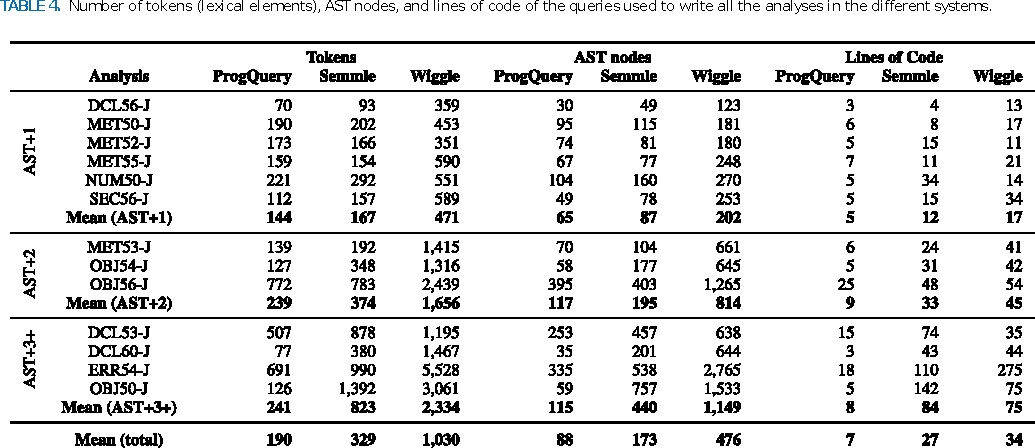
\includegraphics[width=\textwidth]{pictures/ExpressivityOfCypher}
\end{frame}

\begin{frame}[fragile]
  \frametitle{Performance of ProgQuery\footnote{An Efficient and Scalable Platform for Java Source Code Analysis Using Overlaid Graph Representations}}
  \begin{center}
    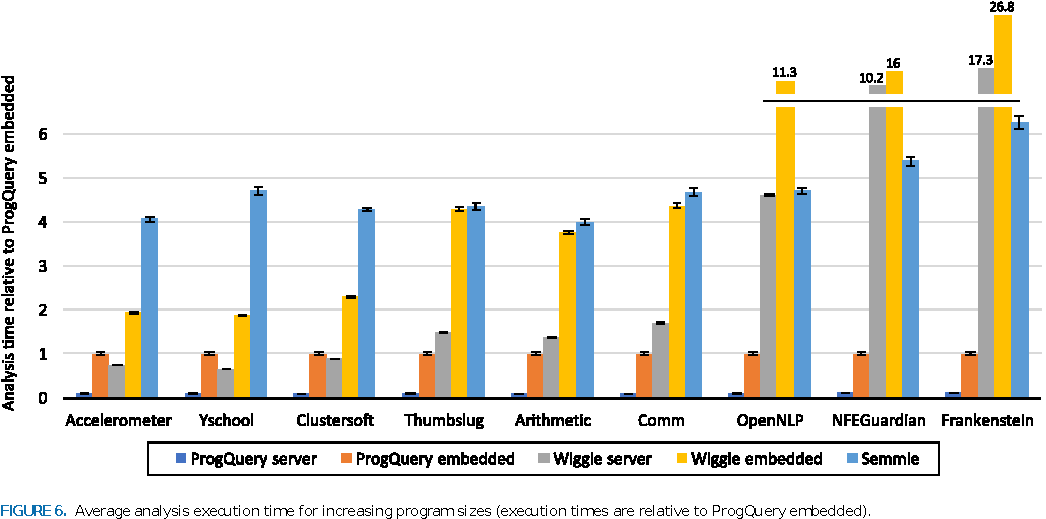
\includegraphics[width=0.9\textwidth]{pictures/Performance}
  \end{center}
\end{frame}

\begin{frame}[fragile]
  \frametitle{Example of Code Analysis in Cypher\footnote{An Efficient and Scalable Platform for Java Source Code Analysis Using Overlaid Graph Representations}}
  \tikzmark{xxx}{} 
  \begin{center}
    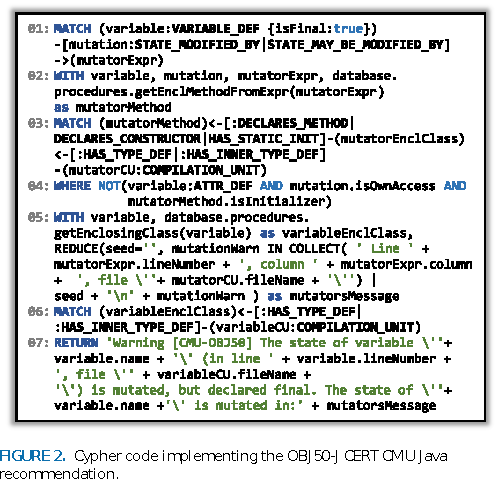
\includegraphics[height=0.8\textheight]{pictures/Example}
  \end{center}
  \pause
  \onslide<2-4>{\tikz[overlay,remember picture]{
    \draw[draw=blue,thick,double,fill opacity=0.2] ($ (xxx) + (4.3,-0.4)$) rectangle ($ (xxx) + (11.0,-3.15)$);
    \draw[draw=blue,thick,double,fill opacity=0.2] ($ (xxx) + (4.3,-4.5)$) rectangle ($ (xxx) + (11.0,-4.99)$);}
    \mycallout<2-4>[opacity=1]{$ (xxx) + (4.4,-0.45)$}{Analysis specification}{3.5}   
    }  
  \onslide<3-4>{\tikz[overlay,remember picture]{
      \draw[draw=red,thick,double,fill opacity=0.2] (A) ($ (xxx) + (4.3,-3.16)$) rectangle ($ (xxx) + (11.0,-4.5)$);
      \draw[draw=red,thick,double,fill opacity=0.2] (B) ($ (xxx) + (4.3,-5.0)$) rectangle ($ (xxx) + (11.0,-6.2)$);}
      \mycallout<3-4>[opacity=1]{$ (xxx) + (4.4,-3.45)$}{Detailed information collection}{5.5}       
      }  
  \onslide<4>{
    \mycallout<4>[opacity=1]{$ (xxx) + (4.4,-4.45)$}{Can we avoid this?}{3.5}      
        }
\end{frame}


\begin{frame}[fragile]
  \frametitle{Conclusion}   
  \begin{itemize}
    \item Datalog-like languages wore widely used in mature tools (for deep code analysis)
    \begin{itemize}
      \item Real-world languages are extensions of Datalog, not pure Datalog: arithmetics, aggregation, algebraic data types, \ldots
      \item Can it be extended more? (\href{https://mgree.github.io/papers/oopsla2020_formulog.pdf}{Formulog: Datalog for SMT-Based Static Analysis})
      \item Datalog is like C++: powerful but too complex for non-familiar users
    \end{itemize}
    \pause
    \item But Cypher can be expressive enough against custom and Datalog-like DSLs
    \begin{itemize}      
      \item Especially for simple checkers specification
      \item Graph database can be an appropriate storage (even Neo4j)
      \item Cypher is like Python: simple, widely-spread but not so powerful
    \end{itemize}
    \pause
    \item There is no production ready solutions for IDE-level declarative code analysis
    \pause
    \item Incremental analysis is a nontrivial challenge
    \pause
    \item Query debugging and results analysis is a nontrivial challenge 
  \end{itemize}
\end{frame}

\begin{frame}[fragile]
  \frametitle{Challenges/Research Directions}  
  \begin{columns}[t]
    \begin{column}{0.5\textwidth}
  \begin{itemize}
    \item Graph databases evaluation
    \begin{itemize}
      \item Code analysis related scenarios
      \item Graph representations comparison
      \item Low-level API comparison  
    \end{itemize}
    \pause
    \item Query languages evaluation
    \begin{itemize}
      \pause
      \item Whether advanced DSL needed?
      \pause
      \item Can GQL be an appropriate language?
      %\pause
      \item GQL is SQL for graphs: \textbf{ISO standard} for graph query language
      %\pause
      \item Cypher-like 
      %\pause
      \item Friendly to non-advanced users, widely used
    \end{itemize}
  \end{itemize}  
 \end{column}
 \pause
\begin{column}{0.5\textwidth}
  \begin{itemize}
    \item Dynamic data analysis
    \begin{itemize}
      \item Incremental view maintenance
      \item Incremental static code analysis
      \item Persistent queries
      \item \ldots
    \end{itemize}
    \pause
    \item Query debugging and results analysis 
    \begin{itemize}
      \item Appropriate data structures
      \item Quick fixes
      \item \ldots
    \end{itemize}
    \item Datalog extensions and Datalog engines
    \begin{itemize}
      \item Performance evaluation
      \item Expressivity comparison
      \item \ldots
    \end{itemize}
  \end{itemize}
\end{column}
\end{columns}
\end{frame}

\end{document}
